\chapter{Validazione statistica e cross-asset}
\label{ch:validazione}

\section{Significatività dei rendimenti}
\label{sec:val-ttest}

Il primo livello di validazione riguarda la significatività statistica dei
rendimenti. Il test $t$ sui rendimenti per trade è significativo all'1\% nel
periodo in-sample ($p = 0{,}007$), mentre nel periodo out-of-sample è
significativo soltanto al 10\% ($p = 0{,}09$): un risultato atteso, dato che
i 10 trade out-of-sample offrono una potenza statistica limitata. La
significatività in-sample, ottenuta attraversando il bear market del 2022, è
il risultato più robusto.

Poiché lo Sharpe ratio è una statistica la cui distribuzione campionaria è
sensibile alla non-normalità dei rendimenti, la sua incertezza è stata
quantificata tramite bootstrap con 10.000 ricampionamenti. Gli intervalli di
confidenza al 95\% risultano $[0{,}72;\,2{,}73]$ in-sample e
$[0{,}25;\,3{,}11]$ out-of-sample; in entrambi i casi l'intervallo non
include lo zero, e la probabilità che lo Sharpe superi l'unità è del 93\%
in-sample e del 90\% out-of-sample. La Figura~\ref{fig:bootstrap} mostra le
due distribuzioni bootstrap.

\begin{figure}[H]
\centering
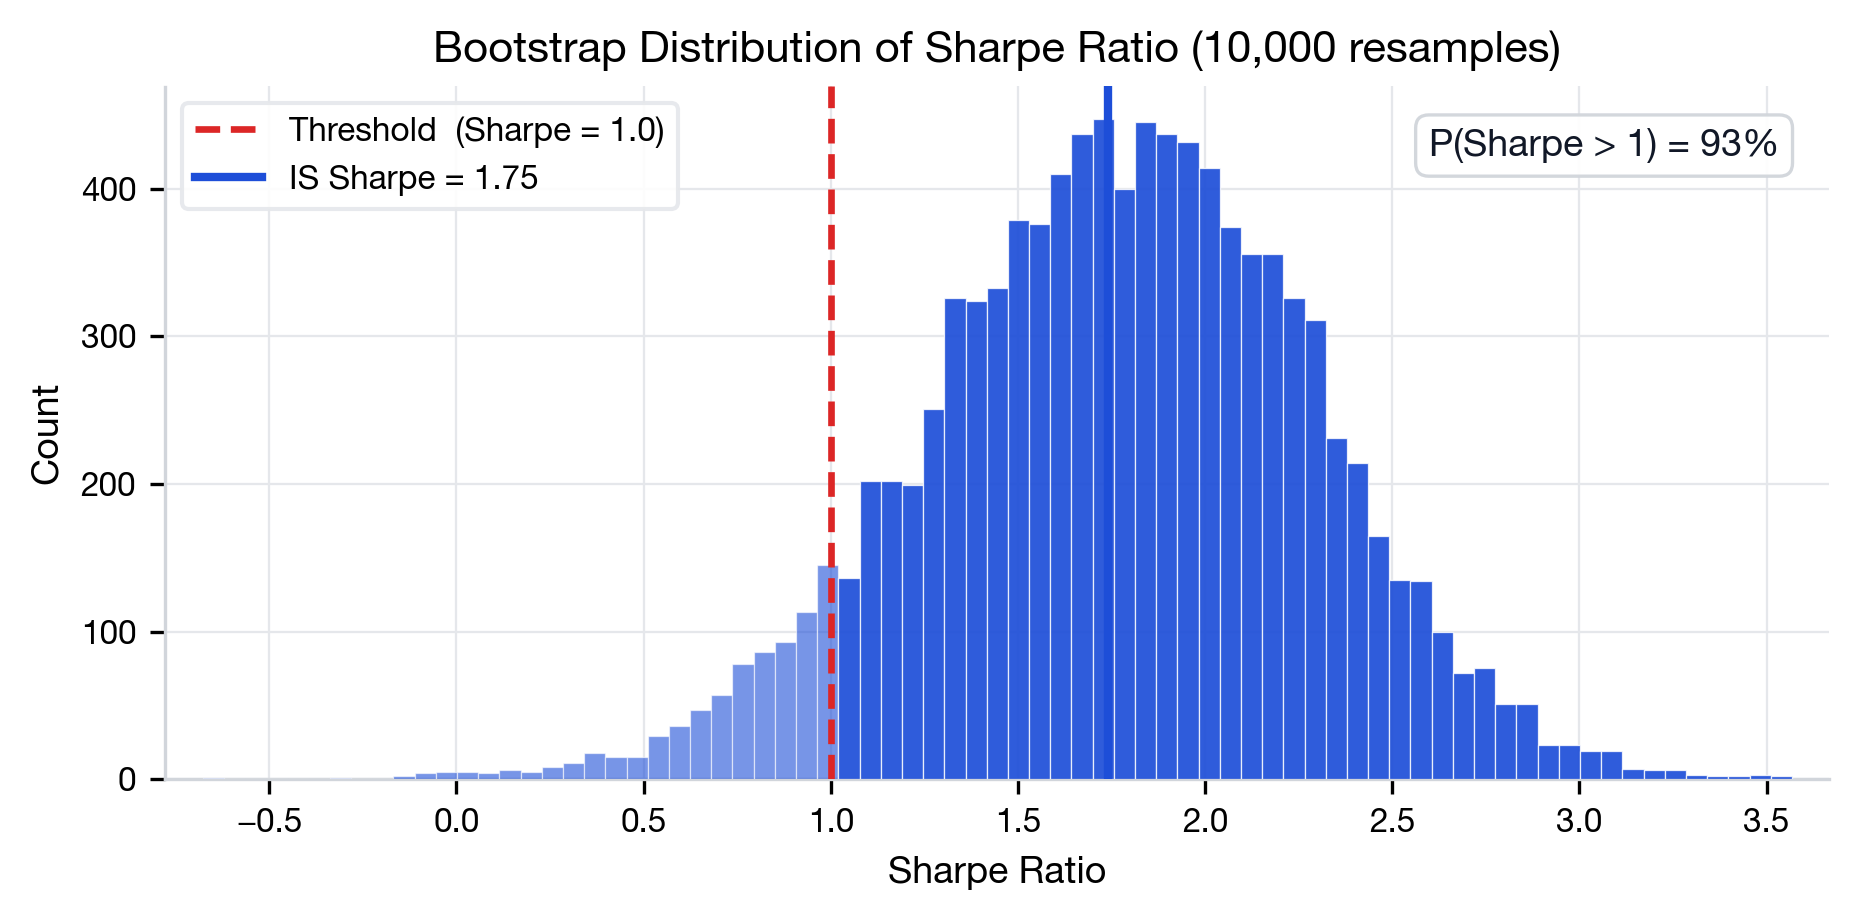
\includegraphics[width=\textwidth]{figures/fig3_bootstrap.png}
\caption{Distribuzione bootstrap dello Sharpe ratio (10.000
ricampionamenti), in-sample e out-of-sample.}
\label{fig:bootstrap}
\end{figure}

\section{Robustezza}
\label{sec:val-robustezza}

Un secondo livello di validazione verifica la robustezza del risultato a
diverse perturbazioni. La prima riguarda la dipendenza da pochi trade
eccezionali: rimuovendo i tre trade più profittevoli, lo Sharpe in-sample
scende a 1,25, restando positivo; rimuovendone cinque, scende a 0,72, ancora
positivo, mentre l'out-of-sample, ridotto a soli cinque trade, non è più
interpretabile. Il risultato in-sample non dipende quindi da un pugno di
osservazioni fortunate.

La seconda perturbazione riguarda i costi. La strategia resta profittevole
anche moltiplicando per dieci i costi di copertura correnti, un margine di
sicurezza ampio rispetto a possibili sottostime dei costi di esecuzione. La
terza riguarda i regimi: coerentemente con la natura di una strategia short
volatility, la performance è forte in regime di volatilità bassa e media e
debole in alta volatilità; sul piano della direzione del mercato, la
strategia funziona sia in fasi rialziste sia ribassiste in-sample (con win
rate del 70\% in entrambe), mentre out-of-sample è forte nelle fasi
rialziste e negativa in quelle laterali. Questo profilo è atteso e coerente
con il meccanismo, non un segno di fragilità.

L'ultima perturbazione riguarda i parametri di uscita. La
Figura~\ref{fig:sensitivity} riporta la griglia di sensibilità sui due
parametri della regola di uscita, il profit target (dal 25\% all'85\%) e la
soglia di giorni a scadenza (da 2 a 10): tutte le 30 combinazioni producono
uno Sharpe positivo (da 0,81 a 2,08) e win rate tra il 48\% e il 70\%. La
combinazione adottata (50\%, 5 giorni) non è un picco isolato della
griglia, ma un punto interno di una regione ampiamente profittevole: la
redditività della strategia non dipende da una scelta fortunata dei
parametri di uscita.

\begin{figure}[H]
\centering
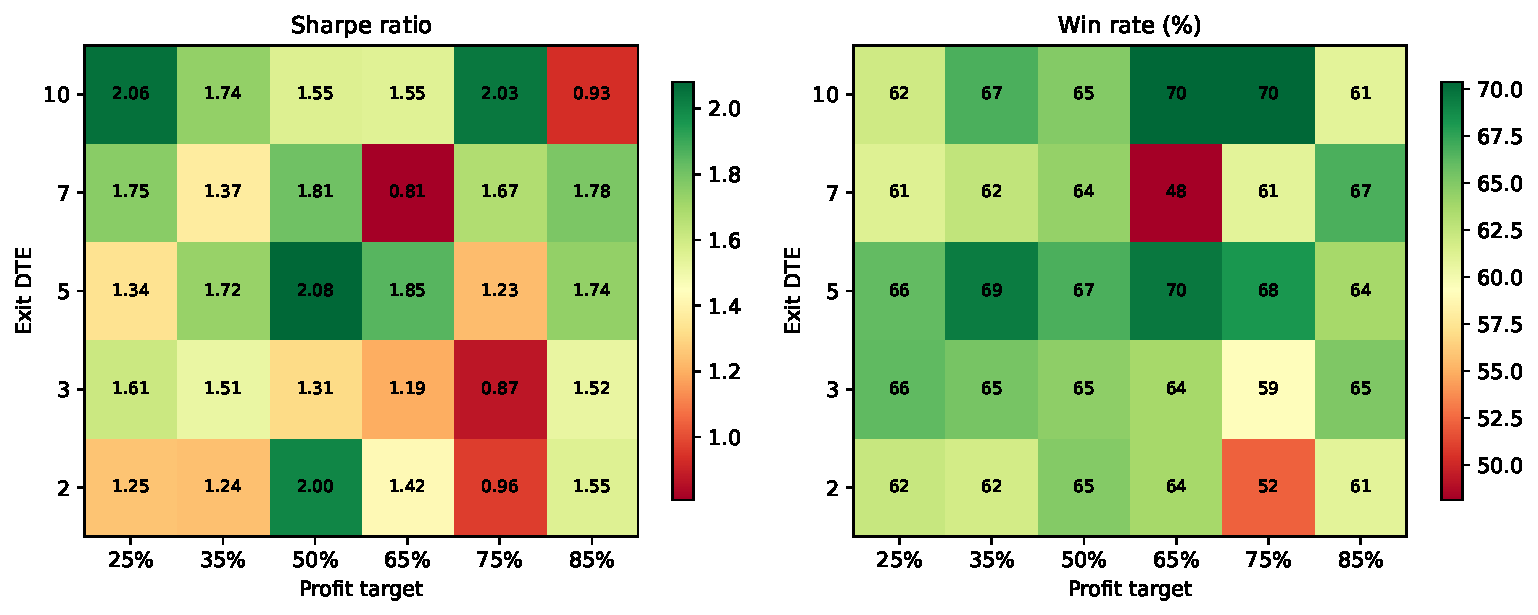
\includegraphics[width=\textwidth]{figures/fig_sensitivity.pdf}
\caption{Analisi di sensibilità sui parametri di uscita: Sharpe ratio (a
sinistra) e win rate (a destra) per ogni combinazione di profit target e
soglia di giorni a scadenza. Tutte le combinazioni sono profittevoli.}
\label{fig:sensitivity}
\end{figure}

\section{Validazione cross-asset: SPY}
\label{sec:val-spy}

Il terzo e più importante livello di validazione affronta il limite
principale del lavoro: la scarsa numerosità del campione Bitcoin. La stessa
strategia Top Vega, con gli stessi parametri e senza alcuna riottimizzazione,
è stata applicata alle opzioni SPY su quattordici anni di dati (147 trade).
L'obiettivo non è proporre una strategia sul mercato azionario, ma verificare
che il meccanismo di cattura del premio non sia un artefatto del campione
Bitcoin.

Due precisazioni metodologiche sulla trasparenza dell'esercizio. Primo,
l'audit dei costi: il primo backtest su SPY utilizzava erroneamente i costi
di Deribit (0,03\% del sottostante per le opzioni, ben superiori ai costi
azionari realistici); dopo la correzione a costi azionari appropriati
(0,65 dollari per contratto sulle opzioni, 0,01 dollari per azione sulla
copertura), il costo per trade è sceso da 140 a 9 dollari e lo Sharpe è
passato da $-0{,}89$ a $+0{,}79$. Secondo, l'audit dei dati: tre record su
9,5 milioni presentavano volatilità implicita negativa, con impatto
complessivo di $-11$ dollari, e non è stato riscontrato alcun artefatto del
tipo prezzo di uscita nullo. La Tabella~\ref{tab:cross-asset} riassume il
confronto.

\begin{table}[H]
\centering
\caption{Confronto cross-asset: la stessa strategia Top Vega su BTC e SPY,
senza riottimizzazione dei parametri.}
\label{tab:cross-asset}
\setlength{\tabcolsep}{4pt}
\begin{tabular}{lccc}
\toprule
\textbf{Metrica} & \textbf{BTC IS (3,3 anni)} & \textbf{BTC OOS (1 anno)} & \textbf{SPY (14 anni)} \\
\midrule
Trade & 35 & 10 & 147 \\
Win rate & 65,7\% & 70,0\% & 66,0\% \\
Sharpe & 1,75 & 1,52 & 0,79 \\
Return & 37,0\% & 14,3\% & 9,1\% \\
Max DD & $-7{,}0\%$ & $-4{,}7\%$ & $-2{,}3\%$ \\
IV media entry & 69\% & n.d. & 16\% \\
Costi/trade & \$100 & n.d. & \$9 \\
\bottomrule
\end{tabular}
\end{table}

Il risultato chiave emerge dalla decomposizione del profitto per trade nelle
sue due componenti, riportata nella Tabella~\ref{tab:decomposizione}.

\begin{table}[H]
\centering
\caption{Decomposizione del profitto per trade: gamba opzionaria contro
copertura. Il win rate della gamba opzionaria è identico sulle due asset
class; la differenza è interamente nell'economia della copertura.}
\label{tab:decomposizione}
\begin{tabular}{lcc}
\toprule
\textbf{Metrica} & \textbf{BTC IS} & \textbf{SPY} \\
\midrule
Win rate option-only & 82,9\% & 82,3\% \\
Win rate totale & 65,7\% & 66,0\% \\
Option PnL/trade & $+\$858$ & $+\$200$ \\
Hedge PnL/trade & $+\$298$ & $-\$129$ \\
\bottomrule
\end{tabular}
\end{table}

\begin{figure}[H]
\centering
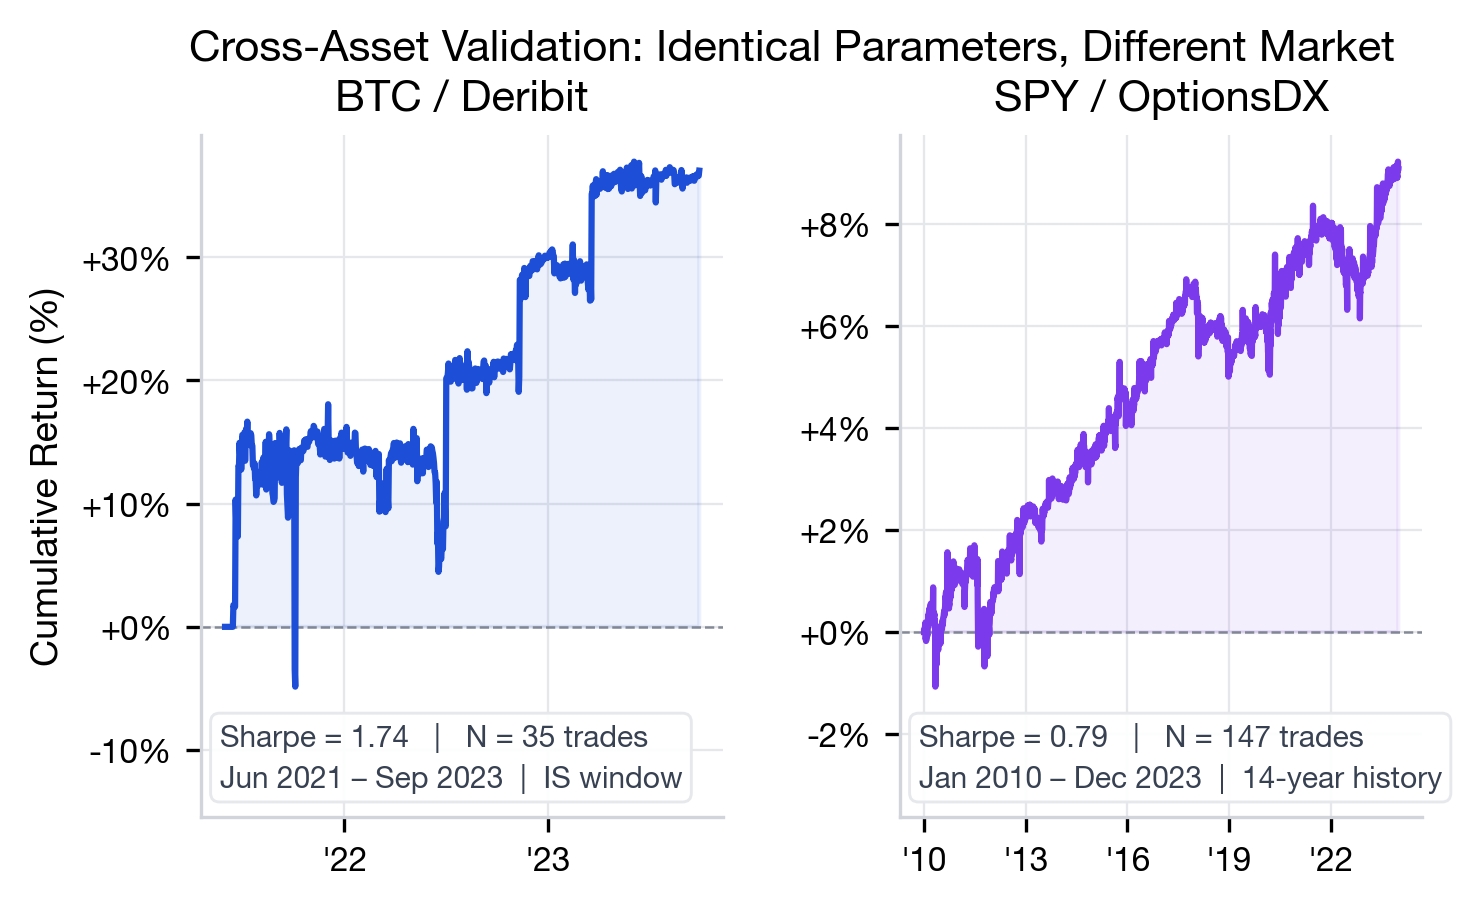
\includegraphics[width=\textwidth]{figures/fig4_crossasset.png}
\caption{Validazione cross-asset su opzioni SPY (2010--2023).}
\label{fig:crossasset}
\end{figure}

La lettura di questi risultati si articola in sei punti.

Primo, il win rate della sola gamba opzionaria è praticamente identico sulle
due asset class (82,9\% su Bitcoin, 82,3\% su SPY): il meccanismo Top Vega
cattura il premio di volatilità con la stessa efficacia su mercati molto
diversi. Questa è la prova centrale che il meccanismo non è specifico di
Bitcoin.

Secondo, la differenza di redditività risiede interamente nella copertura.
Su Bitcoin la copertura guadagna in media 298 dollari per trade, grazie
all'alta volatilità realizzata che rende profittevole il ribilanciamento
gamma; su SPY la copertura perde 129 dollari per trade, perché la volatilità
è troppo bassa e i costi di ribilanciamento superano il profitto da gamma.

Terzo, la verifica che la copertura non abbia un bias direzionale: nei soli
trade con mercato sostanzialmente piatto (rendimento del sottostante
inferiore al 2\% in valore assoluto durante il trade), la copertura su
Bitcoin genera comunque 771 dollari per trade, confermando che il profitto
proviene dal ribilanciamento gamma e non dall'esposizione direzionale; su
SPY, nelle stesse condizioni, la copertura perde 518 dollari per trade,
perché la volatilità realizzata è insufficiente a generare profitto dal
ribilanciamento.

Quarto, l'attribuzione del profitto su Bitcoin: l'81\% del profitto totale
(858 su 1.057 dollari per trade) proviene dalla vendita di opzioni, e il
19\% (298 su 1.057) dalla copertura. La strategia è dunque genuinamente una
raccolta del premio di volatilità; la copertura è un amplificatore del
rendimento su un sottostante ad alta volatilità, non la fonte principale del
profitto.

Quinto, lo Sharpe su Bitcoin è circa doppio rispetto a SPY (1,75 contro
0,79), perché il premio di volatilità su Bitcoin è strutturalmente più ampio,
data una volatilità implicita quattro volte superiore (69\% contro 16\%): il
premio incassato scala con la volatilità, mentre i costi non scalano nella
stessa misura.

Sesto, i 147 trade su quattordici anni compensano la scarsa numerosità del
campione Bitcoin. Un win rate identico (66\%) su un campione quattro volte
più ampio, e su un periodo che comprende la crisi COVID del 2020, il bear
market del 2022 e il ciclo di rialzo dei tassi della Federal Reserve,
conferma che il meccanismo è strutturale e non un artefatto.

È bene ribadire che la validazione su SPY non è presentata come una strategia
azionaria: uno Sharpe di 0,79 e un rendimento del 9,1\% su quattordici anni
non sono attraenti come proposta stand-alone. Il valore dell'esercizio è
dimostrare che il medesimo meccanismo funziona su una asset class diversa, e
che l'alpha è proporzionale al livello della volatilità implicita, il che
individua in Bitcoin, con la sua volatilità strutturalmente elevata, il
mercato in cui il premio è sufficientemente ampio da superare i costi di
copertura.
